\subsection{Sensitivity analysis isolating the equal-variance approximation}\label{app:equal_variance_sensitivity}

For each main simulation scenario, we fixed the component-level marginal distributions and marginal treatment effects and varied only the Gaussian copula latent correlation, $\rho\in\{0,0.2,0.4,0.6,0.8\}$. Within each scenario, the sample size is fixed at the value selected under $\rho=0$ for 85\% WR power. This isolates whether replacing the alternative variance by a null-variance or tie-only equal-variance approximation materially changes the power calculation for WR and NB.

This analysis directly addresses the possibility that the apparent dependence effect could be driven by the equal-variance simplification rather than by dependence itself. For each $\rho$, all formula-based calculations use the same plug-in WR or NB effect size from the simulation summary; only the large-sample variance quantity is changed. Therefore, any difference between the calculated FORSS-$H_A$, FORSS-$H_0$, and Yu--Ganju/Barnhart powers reflects the variance approximation alone, not a change in marginal endpoint effects or in the observed win/loss contrast.

Let $g\in\{WR,NB\}$ index the win measure. For WR, the plug-in effect size is $\widehat{\Delta}_{WR}=\log(\widehat{\tau}_{w,A}/\widehat{\tau}_{l,A})$; for NB, it is $\widehat{\Delta}_{NB}=\widehat{\tau}_{w,A}-\widehat{\tau}_{l,A}$. The FORSS two-variance power approximation used in the main paper is
\begin{align*}
\widehat{\mathrm{Power}}_{A,g}(\rho)
&=
\Phi \left(
\frac{-z_{1-\alpha/2}\sqrt{\widehat{\mathcal A}_{g,0}(\rho)} + \sqrt{m}\,|\widehat{\Delta}_g(\rho)|}
{\sqrt{\widehat{\mathcal A}_{g,A}(\rho)}}
\right).
\end{align*}
Here $m$ is the treatment-arm sample size and $\widehat{\mathcal A}_{g,A}$ and $\widehat{\mathcal A}_{g,0}$ are the FORSS large-sample variance quantities computed from the saved $\Xi$ components under $H_A$ and $H_0$, respectively.
The three power quantities in the formulas below are calculated powers. They are compared with empirical power from trial-level simulation only as an external benchmark.

To isolate the null-variance approximation, we replace the alternative large-sample variance quantity by the null quantity:
\begin{align*}
\widehat{\mathrm{Power}}_{0,g}(\rho)
&=
\Phi \left(
-z_{1-\alpha/2}
+
\frac{\sqrt{m}\,|\widehat{\Delta}_g(\rho)|}
{\sqrt{\widehat{\mathcal A}_{g,0}(\rho)}}
\right).
\end{align*}
The FORSS-$H_0$ calculation is included specifically to assess whether replacing the alternative variance by the null variance, as in an equal-variance planning approximation, changes the power conclusion.

For the Yu--Ganju/Barnhart diagnostic~\cite{yu_sample_2022,barnhart_sample_2025}, we further replace the FORSS variance quantity by the tie-only large-sample variance quantity $\widehat{\mathcal A}_{g,YG}(\rho)$:
\begin{align*}
\widehat{\mathrm{Power}}_{YG,g}(\rho)
&=
\Phi \left(
-z_{1-\alpha/2}
+
\frac{\sqrt{m}\,|\widehat{\Delta}_g(\rho)|}
{\sqrt{\widehat{\mathcal A}_{g,YG}(\rho)}}
\right).
\end{align*}
Since $N=(1+r)m$, where $r=n/m$, the tie-only large-sample variance quantities on the $\mathcal A$-scale are as follows. For $\log(WR)$,
\begin{align*}
\widehat{\mathcal A}_{WR,YG}(\rho)
=
\frac{4\{1+\widehat{\tau}_{\Omega,A}(\rho)\}(1+r)}{3r\{1-\widehat{\tau}_{\Omega,A}(\rho)\}},
\end{align*}
and for NB,
\begin{align*}
\widehat{\mathcal A}_{NB,YG}(\rho)
=
\frac{\{1+\widehat{\tau}_{\Omega,A}(\rho)\}\{1-\widehat{\tau}_{\Omega,A}(\rho)\}(1+r)}{3r}.
\end{align*}

\begin{table}[p]
\centering
\caption{Sensitivity analysis for the null-variance and tie-only variance approximations across the four main simulation scenarios.}
\label{tab:appendix_equal_variance_sensitivity_all}
\setlength{\tabcolsep}{2.1pt}
\scriptsize
\begin{tabular}{@{}ccccccccccc@{}}
\toprule
Measure & $\rho$ & $\widehat{\Delta}$ & $\widehat{\tau}_{\Omega,A}$ & $\widehat{\mathcal A}_0/\widehat{\mathcal A}_A$ & $\widehat{\mathcal A}_{YG}/\widehat{\mathcal A}_0$ & Emp. & $P_A$ & $P_0$ & $P_{YG}$ & $P_0-P_A$ \\
\midrule
\addlinespace[3pt]
\multicolumn{11}{@{}l}{\textbf{S1: Continuous + Continuous ($m=n=274$)}}\\
WR & 0.0 & 0.310 & 0.092 & 0.989 & 1.097 & 85.1 & 85.0 & 85.2 & 81.8 & 0.1 \\
WR & 0.2 & 0.305 & 0.093 & 0.990 & 1.081 & 83.2 & 83.2 & 83.3 & 80.4 & 0.1 \\
WR & 0.4 & 0.308 & 0.099 & 0.991 & 1.064 & 83.0 & 83.0 & 83.2 & 80.8 & 0.1 \\
WR & 0.6 & 0.323 & 0.110 & 0.991 & 1.047 & 85.1 & 84.9 & 85.0 & 83.4 & 0.1 \\
WR & 0.8 & 0.366 & 0.135 & 0.994 & 1.024 & 90.6 & 90.5 & 90.6 & 89.9 & 0.1 \\
NB & 0.0 & 0.140 & 0.092 & 1.024 & 1.107 & 85.4 & 85.2 & 84.9 & 81.2 & -0.3 \\
NB & 0.2 & 0.137 & 0.093 & 1.024 & 1.090 & 83.6 & 83.3 & 83.0 & 79.7 & -0.3 \\
NB & 0.4 & 0.138 & 0.099 & 1.024 & 1.074 & 83.4 & 83.2 & 82.9 & 80.2 & -0.3 \\
NB & 0.6 & 0.142 & 0.110 & 1.026 & 1.059 & 85.4 & 85.1 & 84.8 & 82.7 & -0.3 \\
NB & 0.8 & 0.156 & 0.135 & 1.030 & 1.045 & 90.8 & 90.8 & 90.5 & 89.3 & -0.3 \\
\addlinespace[3pt]
\multicolumn{11}{@{}l}{\textbf{S2: Continuous + Binary ($m=n=269$)}}\\
WR & 0.0 & 0.363 & 0.229 & 1.012 & 1.077 & 85.8 & 85.0 & 84.9 & 82.2 & -0.1 \\
WR & 0.2 & 0.349 & 0.232 & 1.012 & 1.067 & 82.8 & 81.7 & 81.6 & 79.1 & -0.1 \\
WR & 0.4 & 0.340 & 0.241 & 1.012 & 1.057 & 79.6 & 78.5 & 78.3 & 76.1 & -0.1 \\
WR & 0.6 & 0.334 & 0.256 & 1.011 & 1.049 & 76.4 & 75.4 & 75.3 & 73.3 & -0.1 \\
WR & 0.8 & 0.335 & 0.285 & 1.007 & 1.043 & 73.7 & 72.7 & 72.6 & 70.8 & -0.1 \\
NB & 0.0 & 0.138 & 0.229 & 1.012 & 1.132 & 86.1 & 86.0 & 85.9 & 81.4 & -0.1 \\
NB & 0.2 & 0.133 & 0.232 & 1.009 & 1.119 & 83.0 & 82.8 & 82.7 & 78.3 & -0.1 \\
NB & 0.4 & 0.128 & 0.241 & 1.006 & 1.109 & 79.9 & 79.6 & 79.5 & 75.3 & -0.1 \\
NB & 0.6 & 0.123 & 0.256 & 1.003 & 1.100 & 76.7 & 76.5 & 76.5 & 72.5 & -0.0 \\
NB & 0.8 & 0.119 & 0.285 & 0.999 & 1.093 & 74.0 & 73.8 & 73.8 & 70.0 & 0.0 \\
\addlinespace[3pt]
\multicolumn{11}{@{}l}{\textbf{S3: Survival + Continuous ($m=n=239$)}}\\
WR & 0.0 & 0.356 & 0.129 & 0.951 & 1.047 & 84.0 & 85.1 & 85.7 & 84.0 & 0.6 \\
WR & 0.2 & 0.339 & 0.131 & 0.953 & 1.048 & 80.6 & 81.6 & 82.2 & 80.4 & 0.6 \\
WR & 0.4 & 0.326 & 0.135 & 0.955 & 1.051 & 77.2 & 78.3 & 78.8 & 76.8 & 0.5 \\
WR & 0.6 & 0.314 & 0.142 & 0.956 & 1.054 & 73.9 & 74.8 & 75.3 & 73.1 & 0.5 \\
WR & 0.8 & 0.306 & 0.155 & 0.957 & 1.059 & 70.6 & 71.7 & 72.2 & 69.7 & 0.4 \\
NB & 0.0 & 0.153 & 0.129 & 1.037 & 1.016 & 84.3 & 84.3 & 83.8 & 83.3 & -0.4 \\
NB & 0.2 & 0.146 & 0.131 & 1.034 & 1.016 & 81.1 & 80.7 & 80.3 & 79.6 & -0.4 \\
NB & 0.4 & 0.140 & 0.135 & 1.032 & 1.017 & 77.6 & 77.1 & 76.8 & 76.1 & -0.4 \\
NB & 0.6 & 0.133 & 0.142 & 1.031 & 1.019 & 74.3 & 73.5 & 73.2 & 72.4 & -0.3 \\
NB & 0.8 & 0.128 & 0.155 & 1.030 & 1.024 & 71.1 & 70.3 & 70.0 & 69.0 & -0.3 \\
\addlinespace[3pt]
\multicolumn{11}{@{}l}{\textbf{S4: Binary + Continuous ($m=n=239$)}}\\
WR & 0.0 & 0.398 & 0.229 & 1.004 & 1.010 & 85.6 & 85.1 & 85.1 & 84.7 & -0.0 \\
WR & 0.2 & 0.379 & 0.232 & 1.005 & 1.012 & 81.9 & 81.4 & 81.3 & 80.9 & -0.1 \\
WR & 0.4 & 0.363 & 0.241 & 1.006 & 1.016 & 78.2 & 77.5 & 77.4 & 76.8 & -0.1 \\
WR & 0.6 & 0.351 & 0.256 & 1.006 & 1.022 & 74.2 & 73.4 & 73.4 & 72.5 & -0.1 \\
WR & 0.8 & 0.343 & 0.285 & 1.005 & 1.032 & 70.3 & 69.3 & 69.3 & 67.9 & -0.0 \\
NB & 0.0 & 0.151 & 0.229 & 1.013 & 1.062 & 85.9 & 86.1 & 85.9 & 83.8 & -0.2 \\
NB & 0.2 & 0.144 & 0.232 & 1.009 & 1.063 & 82.2 & 82.4 & 82.3 & 79.9 & -0.1 \\
NB & 0.4 & 0.136 & 0.241 & 1.006 & 1.066 & 78.6 & 78.5 & 78.5 & 75.9 & -0.1 \\
NB & 0.6 & 0.129 & 0.256 & 1.003 & 1.072 & 74.6 & 74.6 & 74.5 & 71.6 & -0.0 \\
NB & 0.8 & 0.122 & 0.285 & 0.999 & 1.082 & 70.7 & 70.4 & 70.4 & 67.0 & 0.0 \\
\bottomrule
\end{tabular}
\parbox{0.96\textwidth}{\footnotesize \textit{Note:} $\widehat{\Delta}$ denotes the plug-in effect size under $H_A$, and $\widehat{\tau}_{\Omega,A}$ denotes the plug-in overall tie probability under $H_A$. $P_A$ denotes the standard FORSS two-variance power calculation, $P_0$ denotes the FORSS null-variance calculation, and $P_{YG}$ denotes the Yu--Ganju/Barnhart tie-only calculation. The ratios $\widehat{\mathcal A}_0/\widehat{\mathcal A}_A$ and $\widehat{\mathcal A}_{YG}/\widehat{\mathcal A}_0$ quantify, respectively, the null-variance substitution relative to the full FORSS large-sample variance quantity and the tie-only approximation relative to the null large-sample variance quantity. Power values and $P_0-P_A$ are reported as percentages and percentage points, respectively. Emp. is the trial-level simulation benchmark. Source summaries: S1: \texttt{Summary.Scenario1.Nsp2000.csv}; S2: \texttt{Summary.Scenario2.Nsp2000.csv}; S3: \texttt{Summary.Scenario3.Nsp2000.csv}; S4: \texttt{Summary.Scenario4.Nsp2000.csv}.}
\end{table}

The numerical results in Table~\ref{tab:appendix_equal_variance_sensitivity_all}, together with the graphical summary in Figure~\ref{fig:appendix_equal_variance_sensitivity_all}, show that replacing the alternative variance by the null variance has a limited effect on the calculated power compared with the empirical power changes induced by increasing dependence. For WR, the FORSS-$H_0$ minus FORSS-$H_A$ power difference ranged from about $-0.1$ to 0.6 percentage points across all scenarios and correlations; for NB, the corresponding range was about $-0.4$ to 0.0 percentage points. Moreover, the direction was not uniformly conservative: the null-variance substitution increased WR power in S1 and S3, but decreased WR power in S2 and S4, while it generally decreased NB power. Thus, the large power losses seen under independence-based planning in S2--S4 cannot be attributed to the equal-variance approximation. They arise primarily because increasing dependence changes the overall win/loss contrast itself.

\begin{figure}[p]
\centering
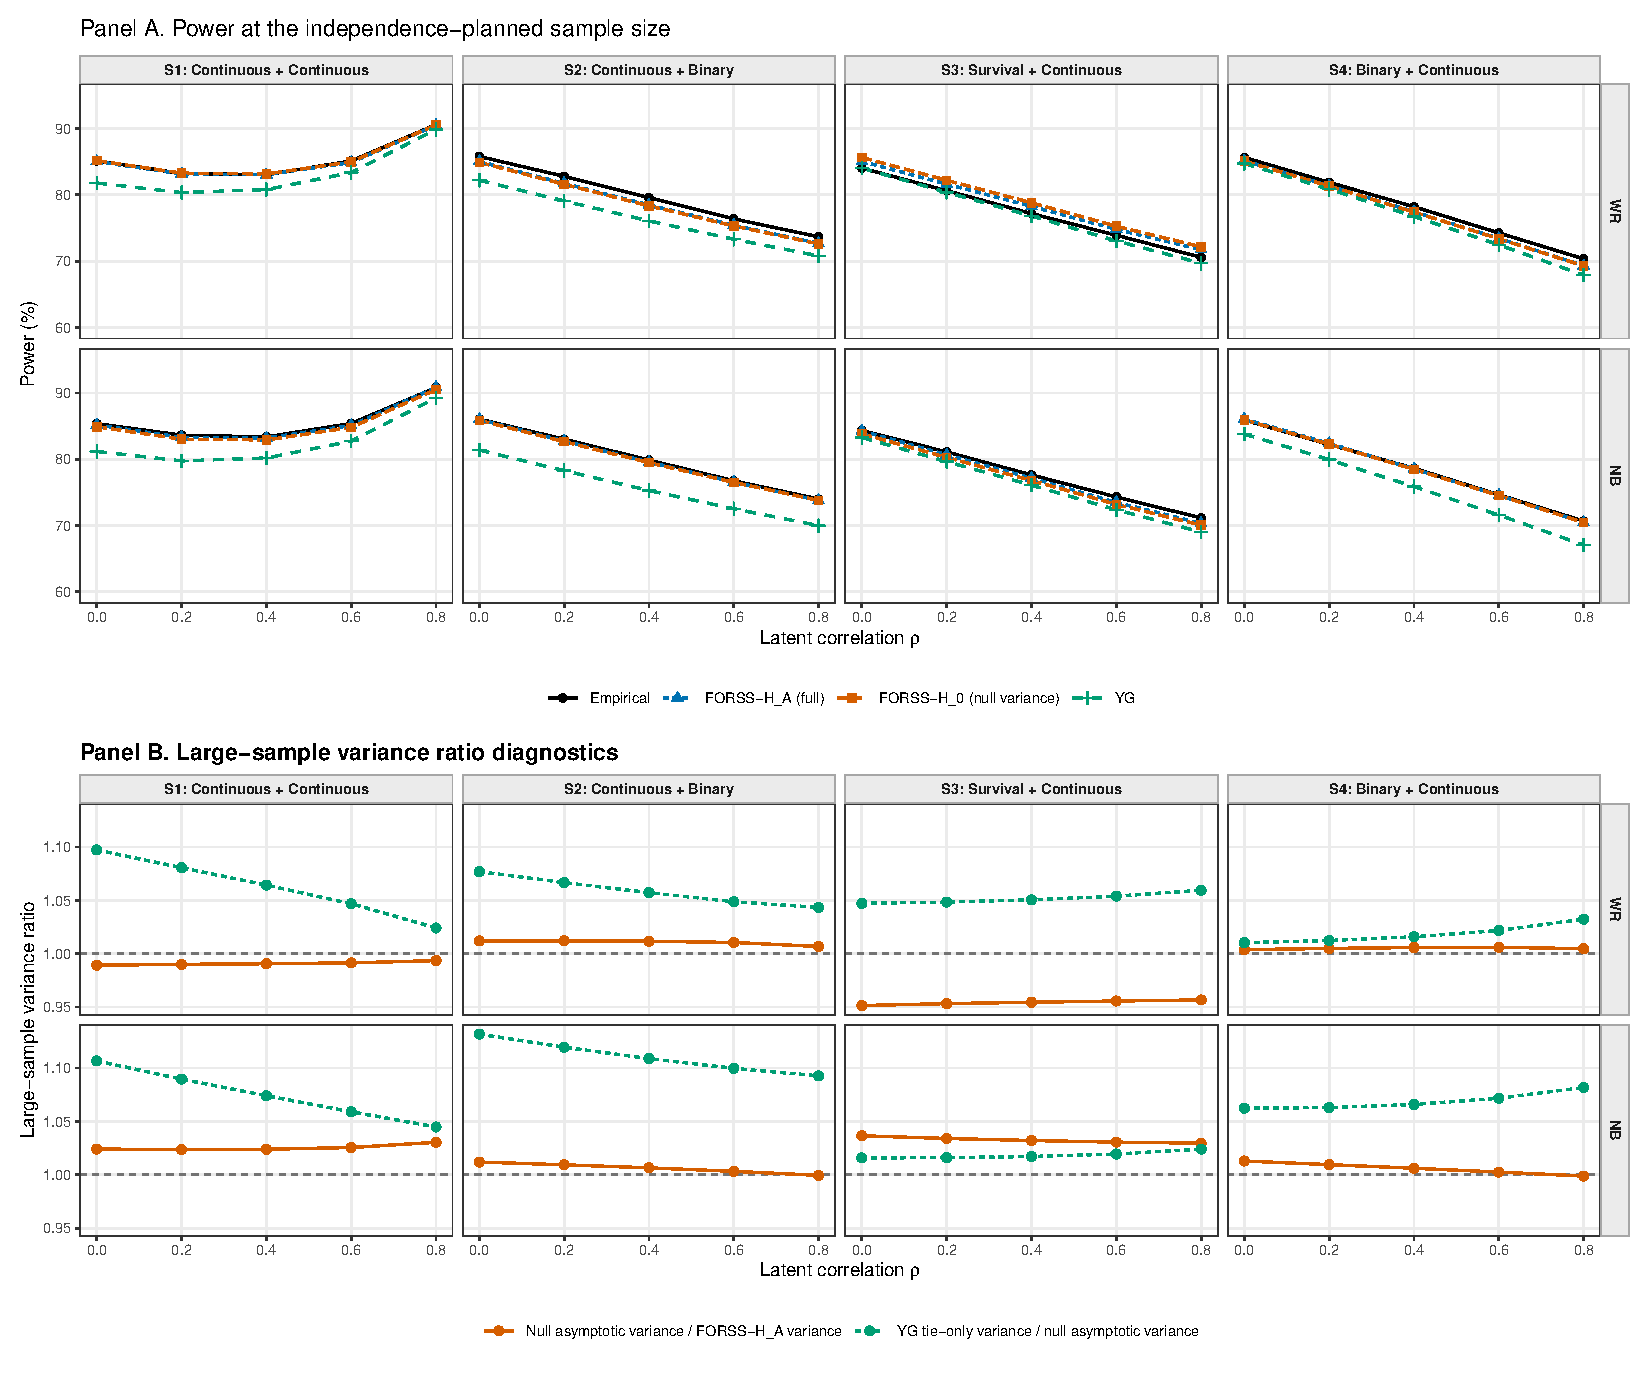
\includegraphics[width=0.98\textwidth]{Simulation Examples/Appendix.EqualVarianceSensitivity.AllScenarios.pdf}
\caption{Sensitivity analysis for the null-variance and tie-only variance approximations. Panel A compares empirical power with three calculated powers: the full FORSS two-variance calculation (FORSS-$H_A$), the null-variance approximation (FORSS-$H_0$), and the Yu--Ganju/Barnhart tie-only approximation at the sample size selected under $\rho=0$. Panel B displays the ratios $\widehat{\mathcal A}_0(\rho)/\widehat{\mathcal A}_A(\rho)$ and $\widehat{\mathcal A}_{YG}(\rho)/\widehat{\mathcal A}_0(\rho)$, which quantify the extent of the null-variance substitution and the tie-only approximation relative to the null large-sample variance quantity.}
\label{fig:appendix_equal_variance_sensitivity_all}
\end{figure}
